\documentclass[12pt]{article}
\pagenumbering{gobble}

\usepackage{amsmath}
\usepackage{amsfonts}
\usepackage{amssymb}
\usepackage{fancyhdr}
\usepackage[headheight=0.25in,margin=1in]{geometry}

\usepackage{tikz}

\newcommand{\parens}[1]{\left( #1 \right)}

\newcommand{\N}{\mathbb{N}}
\newcommand{\Z}{\mathbb{Z}}
\newcommand{\Q}{\mathbb{Q}}
\newcommand{\R}{\mathbb{R}}
\newcommand{\C}{\mathbb{C}}

\newcommand{\solution}{\textbf{Solution:}}
\newcommand{\proof}{\textbf{Proof:}}
\newcommand{\done}{\ensuremath{
    \strut\hfill\blacksquare
}}

\linespread{1.25}

\begin{document}
    \pagestyle{fancy}

    \fancyhead[L]{Computer Networks}
    \fancyhead[C]{Lab 1 - Protocol Stack}
    \fancyhead[R]{Alex Agruso}

    \begin{itemize}
        \item [Step 3.)] Frame 18, HTTP/GET Packet:
        \begin{center}
            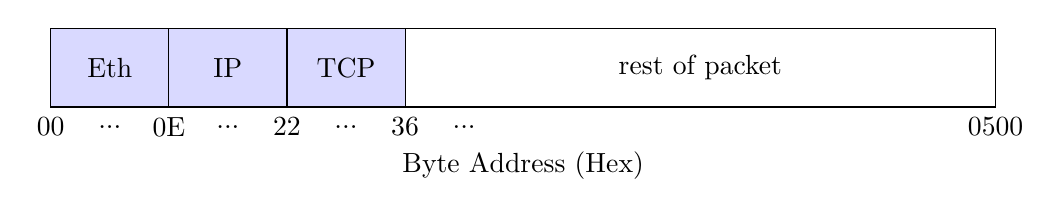
\begin{tikzpicture}
                \draw[] (0,0) rectangle (12,1);
                \node[] at (6,-0.75) {Byte Address (Hex)};

                \node[] at (0,-0.25) {00};
                \node[] at (0.75,-0.25) {...};
                \draw[fill=blue!15!white] (0,0) rectangle (1.5,1)
                    node[midway] {Eth};

                \node[] at (1.5,-0.25) {0E};
                \node[] at (2.25,-0.25) {...};
                \draw[fill=blue!15!white] (1.5,0) rectangle (3,1)
                    node[midway] {IP};

                \node[] at (3,-0.25) {22};
                \node[] at (3.75,-0.25) {...};
                \draw[fill=blue!15!white] (3,0) rectangle (4.5,1)
                    node[midway] {TCP};

                \node[] at (4.5,-0.25) {36};
                \node[] at (5.25,-0.25) {...};
                \draw[] (4.5,0) rectangle (12,1)
                    node[midway] {rest of packet};

                \node[] at (12,-0.25) {0500};
            \end{tikzpicture}
        \end{center}

        \item [Step 4.)] Looking at the download packets, we find that each has
        a download protocol overhead (ethernet, IP, and TCP) of 54 bytes.
        In each packet, ethernet is 14 bytes in length, while IP and TCP are
        both 20 bytes in length.
        
        Taking the average of the total lengths of each download packet to be
        1,425 bytes, we find the average download protocol overhead to be
        \[
            \frac{\text{overhead}}{\text{average total length}}
            = \frac{54 \ \text{bytes}}{1,425 \ \text{bytes}}
            = 0.0378
            = 3.78\%
            ,
        \]
        thus a good estimate for the download protocol overhead would be about
        54 bytes, or about 4\% of the total packet length. Considering how messages
        are usually larger than a kilobyte, a 50 byte overhead seems insignificant.

        \item [Step 5.1.)] The demultiplexing key for ethernet is
        ``\verb|Type|'', which takes the value ``\verb|IPv4|'' in order to
        indicate that we are using the IP protocol.

        \item [Step 5.2.)] The demultiplexing key for IP is ``\verb|Protocol|'',
        which takes the value ``\verb|TCP|'' in order to indicate that we are
        using TCP.
    \end{itemize}
\end{document}
